% !TeX program = xelatex
% !TeX spellcheck = en_CA
% !TeX encoding = utf8

\documentclass[10pt,landscape,letterpaper]{article}

%
% formula-sheet.tex
%
% My formula sheet for use during Mec E 230 (Thermofluids
% Formula sheet based off of this template:


\usepackage{multicol}
\usepackage{calc}
\usepackage{ifthen}
\usepackage[landscape,letterpaper]{geometry}
\usepackage{titlesec}
\usepackage{amsmath,amsthm,amsfonts,amssymb,gensymb,nicefrac}
\usepackage{graphicx,overpic,wrapfig}
\usepackage[dvipsnames]{xcolor}

\usepackage{fontspec}
\usepackage{newtxtext, newtxmath}

\usepackage[pdfauthor={Johann M. Barnard},
            pdftitle={Mec E 230 Formula Sheet},
            pdfsubject={Mec E 230},
            pdfkeywords={LaTeX, XeLaTeX, Mec E 230, Formula Sheet},
            pdfproducer={XeLaTeX with hyperref},
            pdfcreator={XeLaTeX}]{hyperref}
            
\usepackage{siunitx}
\sisetup{inter-unit-product=\ensuremath{{}\cdot{}}}
\sisetup{per-mode=fraction}

% We need some custom, non-SI units so we'll declare those here:
\DeclareSIUnit{\slug}{slug}
\DeclareSIUnit{\pounds}{lb}
\DeclareSIUnit{\poundsforce}{\pounds f}
\DeclareSIUnit{\poundsmass}{\pounds m}
\DeclareSIUnit{\poundsmole}{\pounds mol}
\DeclareSIUnit{\britishthermal}{Btu}
\DeclareSIUnit{\rankine}{R}
\DeclareSIUnit{\feet}{ft}
\DeclareSIUnit{\PressurePerSquareInch}{psi}
\DeclareSIUnit{\AbsPressurePerSquareInch}{\PressurePerSquareInch a}
\DeclareSIUnit{\degreeFahrenheit}{\degree F}

\graphicspath{{./}}

% This sets page margins to .5 inch if using letter paper, and to 1cm
% if using A4 paper. (This probably isn't strictly necessary.)
% If using another size paper, use default 1cm margins.
\ifthenelse{ \lengthtest { \paperwidth = 11in}}
    {\geometry{top=.5in,left=.5in,right=.5in,bottom=.5in}}
    {\ifthenelse{ \lengthtest{ \paperwidth = 297mm}}
        {\geometry{top=1cm,left=1cm,right=1cm,bottom=1cm}}
        {\geometry{top=1cm,left=1cm,right=1cm,bottom=1cm}}
    }

% Turn off header & footer
\pagestyle{empty}

% Redefine section commands to use less space
\makeatletter
\renewcommand{\section}{\@startsection{section}{1}{0mm}%
                                {-1ex plus -.5ex minus -.2ex}%
                                {0.5ex plus .2ex}%x
                                {\normalfont\large\bfseries}}
\renewcommand{\subsection}{\@startsection{subsection}{2}{0mm}%
                                {-1ex plus -.5ex minus -.2ex}%
                                {0.5ex plus .2ex}%
                                {\normalfont\normalsize\bfseries}}
\renewcommand{\subsubsection}{\@startsection{subsubsection}{3}{0mm}%
                                {-1ex plus -.5ex minus -.2ex}%
                                {1ex plus .2ex}%
                                {\normalfont\small\bfseries}}
\makeatother

\titlespacing*{\section}{0pt}{0.5ex}{0.25ex}
\titlespacing*{\subsection}{0pt}{0.5cm}{0.25cm}

% Figure fix. See https://tex.stackexchange.com/a/12289
\newenvironment{Figure}
    {\par\medskip\noindent\minipage{\linewidth}}
    {\endminipage\par\medskip}

% Define BibTeX command
\def\BibTeX{{\rm B\kern-.05em{\sc i\kern-.025em b}\kern-.08em
  T\kern-.1667em\lower.7ex\hbox{E}\kern-.125emX}}

% Define shortcut for formatting equation labels:
\definecolor{FSheetLabelColor}{RGB}{245, 82, 73}
\newcommand{\fsheetlabel}[1]{\textcolor{FSheetLabelColor}{\textbf{\textit{#1}}}}

% Don't print section numbers
\setcounter{secnumdepth}{0}


\setlength{\parindent}{0pt}
\setlength{\parskip}{0pt plus 0.5ex}

%My Environments
\newtheorem{example}[section]{Example}
% -----------------------------------------------------------------------

\begin{document}
    \raggedright
    \footnotesize
    \begin{multicols*}{3}
    
    
    % multicol parameters
    % These lengths are set only within the two main columns
    % \setlength{\columnseprule}{0.25pt}
    \setlength{\premulticols}{1pt}
    \setlength{\postmulticols}{1pt}
    \setlength{\multicolsep}{1pt}
    \setlength{\columnsep}{2pt}
    
    \begin{center}
        \Large{\underline{Mec E 230 Formula Sheet}} \\
    \end{center}
    
    %--------------------------------------
    \begin{minipage}{\columnwidth}\raggedright
        \subsection{Generalized CV-CS Analysis}
        
        \fsheetlabel{Conservation of mass:} $\frac{dm_{CV}}{dt} = \dot{m}_{in} - \dot{m}_{out}$
        
        \fsheetlabel{Conservation of energy:} $$\frac{dE_{CV}}{dt} = (\dot{E}_{in} - \dot{E}_{out}) + (\dot{W}_{in} - \dot{W}_{out}) + \dot{Q} - \dot{W}\text{,}$$ where for \textbf{Closed system} $\Rightarrow$ no mass in/out of system, \textbf{steady-state system} $\Rightarrow$ no $\Delta$ w/ time, \textbf{adiabatic system} $\Rightarrow$ no addition/removal of heat.
    \end{minipage}
    \vspace{2ex plus .5ex minus .5ex}
    %--------------------------------------
    
    %--------------------------------------
    \begin{minipage}{\columnwidth}\raggedright
        \subsection{Work}
        
        \fsheetlabel{General:} $W = \int F \,dx$
        
        \fsheetlabel{Translational:} $W_{M,T} = \int_{s_1}^{s_2} F\,ds$ and $\dot{W}_{M,T} = Fv$. \\*
        $F$, $s$, and $v$ are in the same direction.
        
        \fsheetlabel{Rotational:} $W_{M,R} = \int_{\theta_1}^{\theta_2} T\,d\theta$ and $\dot{W}_{M,R} = T\omega$.
        
        \fsheetlabel{Electrical:} $W_E = \int_{t_1}^{t_2} \xi I \,dt$ and $\dot{W}_E = \xi I$.
        
        \fsheetlabel{Boundary:} $W_B = \int_{V_1}^{V_2} p\,dV$.
        
        \fsheetlabel{Flow:} $\dot{W}_F = \dot{m}w_F$, where $w_F = p \nu = \frac{p}{\rho}$
        
        \subsubsection{Change in the energy in a system}
        
        \begin{equation*}
            \Delta E_{CV} = \Delta KE + \Delta PE + \Delta U_T + \Delta U_L + \Delta U_C + \Delta U_N
        \end{equation*}
        
        where:
        
        \begin{itemize}
            \item $\Delta KE = \frac{1}{2}\left(m\left(v_2^2 - v_1^2) + I_G(\omega_2^2 + \omega_1^2\right)\right)$
            
            \item $\Delta PE = mg(h_2 - h_1)$
            
            \item $\Delta U_T = m \int_{T_1}^{T_2} c_v(T) \,dT$ where if ${c_v}$ is constant we write $\Delta U_T = mc_v(T_2-T_1)$
            
            \item $\Delta U_L = mu_L$ where $u_L$ is the specific latent heat of phase change.
        \end{itemize}
    \end{minipage}
    \vspace{2ex plus .5ex minus .5ex}
    %--------------------------------------
    
    %--------------------------------------
    \begin{minipage}{\columnwidth}\raggedright
        \subsection{Random heat/pressure-related things}
        
        \fsheetlabel{Adiabatic, quasi-equilibrium, ideal gas, const. $c_{v}$:} $\frac{T_2}{T_1} = \left(\frac{V_1}{V_2}\right)^{k-1}$; $\frac{p_2}{p_1} = \left(\frac{V_1}{V_2}\right)^{k-1}$, where $k$ is a constant from table A-8 or table B-8.
        
        \fsheetlabel{Pressure:} $p=\frac{1}{3} m_p \hat{n} \left\langle v^2 \right\rangle$ where $m_p$ is the mass of the particle, $\hat{n}$ is the number of particles per unit volume, and $v$ is the particle's velocity.
        
        Also, \fsheetlabel{pressure:} $p=\frac{F}{A}$.
        
        \fsheetlabel{Ideal Gas Law:} $pV=n\bar{R}T$
        
        \fsheetlabel{Moles $\Leftrightarrow$ Mass:} $m = nM$
        
        \fsheetlabel{Specific volume:} $\nu = \frac{1}{\rho} = \frac{V}{m}$
        
        \fsheetlabel{Isothermal:} $V_1 p_1 = V_2 p_2$ since $nRT$ is constant.
    \end{minipage}
    \vspace{2ex plus .5ex minus .5ex}
    %--------------------------------------
    
    %--------------------------------------
    \begin{minipage}{\columnwidth}\raggedright
        \subsection{Random notes}
        
        \fsheetlabel{3 (+ 1?) types of piston problems:}
        
        \begin{enumerate}
            \item \textbf{Isothermal}: $T$ is constant, $p$ varies. So replace $p$ with something like $\frac{p_1 V_1}{V}$ in your $W_B$ integral.
            \item \textbf{Isobaric}: $T$ varies, $p$ is constant.
            \item \textbf{Nothing constant, but adiabatic}: Remeber that $pV^n = constant$, where $n$ is given to you. Should be able to derive something like $W = \frac{m c_v}{R}(p_1 V_1 - p_2 V_2)$.
            \item \textbf{Isotropic}: Same as Isothermal, but replace $p$ with something like $\frac{p_1 V_1^n}{V^n}$ instead.
        \end{enumerate}
    \end{minipage}
    \vspace{2ex plus .5ex minus .5ex}
    %--------------------------------------
    
    %--------------------------------------
    \begin{minipage}{\columnwidth}\raggedright
        \subsection{Heat transfer}
        
        \fsheetlabel{Conduction (Fourier's law (1D)):} $\dot{Q}_{cond} = -kA\frac{dT}{dx}$
        
        Then, if $k$ and $A$ are constant with $x$: $\left|\dot{Q}_{cond}\right| = -\frac{kA}{L} \Delta T = \frac{1}{R_{cond}} \Delta T$, where $R_{cond} = \frac{L}{kA}$.
        
        For \fsheetlabel{heat transfer through the walls of a cylinder} (e.g. pipe), $A$ is not constant w.r.t. $r$, and $\left|\dot{Q}_{cond}\right| = \frac{1}{R_{cond}} \Delta T$ where $R_{cond} = \frac{\ln\left(r_{outer}/r_{inner}\right)}{2 \pi L k}$, with $L$ being the length of the pipe.
        
        \fsheetlabel{Equivalent resistances:}\\*
        Series: $R_{eff}=R_1+R_2$; Parallel: $\frac{1}{R_{eff}} = \frac{1}{R_1} + \frac{1}{R_2}.$
        
        \fsheetlabel{Convective resistance:} $R_{conv} = \frac{1}{hA}$
    \end{minipage}
    \vspace{2ex plus .5ex minus .5ex}
    %--------------------------------------
    
    %--------------------------------------
    \begin{minipage}{\columnwidth}\raggedright
        \subsection{Lumped-system approximation}
        
        \fsheetlabel{Valid if} $Bi<0.1$, where $Bi=\frac{L_s h_f}{k_s}$ and $L_s = \frac{V}{A}$.
        
        \fsheetlabel{Then}, $$\frac{T(t) - T_f}{T(0) - T_f} = e^{-\frac{h}{\rho c_v L_s}t},$$ $$t = -\frac{\rho c_v L_s}{h} \ln{\left(\frac{T(t) - T_f}{T(0) - T_f)}\right)},$$ and $$T(t) = T_f + \left(T(0) - T_f\right) e^{-\frac{h}{\rho c_v L_s}t}$$
        
        Note that the fraction $\frac{h}{\rho c_v L_s}$ is sometimes called the \textbf{time constant of cooling / heating}.
    \end{minipage}
    \vspace{2ex plus .5ex minus .5ex}
    %--------------------------------------
    
    %--------------------------------------
    \begin{minipage}{\columnwidth}\raggedright
        \subsection{Fluid mechanics}
        
        \fsheetlabel{General shear stress:} $\tau = \tau_0 + \mu (\frac{dv}{dy})^n$, where $\mu$ is \textbf{dynamic viscosity} and $\nu = \frac{\mu}{\rho}$ is \textbf{kinematic viscosity}.
        
        \fsheetlabel{Fluid types:}
        
        \begin{itemize}
            \item \textbf{Newtonian}: $\tau_0 = 0$, $n = 1$; Most fluids, linear relationship between shear stress and strain.
            
            \item \textbf{Bingham plastic}: $\tau_0 \neq 0$, $n = 1$; Requires some force to start flow, e.g. ketchup, toothpaste.
            
            \item \textbf{Shear-thinning}: $\tau_0 = 0$, $n < 1$; Can accelerate without effort when shear reaches critical value, e.g. blood.
            
            \item \textbf{Shear-thickening}: $\tau_0 = 0$, $n > 1$; Liquid under slow \& steady force, solid under sudden force, e.g. cornstarch in water.
        \end{itemize}
    
        \fsheetlabel{Density:} $\rho=\frac{m}{V}$. \fsheetlabel{Specific volume:} $\nu=\frac{1}{\rho}$. 
        
        \fsheetlabel{Specific gravity:} $SG = \frac{\rho_{thing}}{\rho_{H_2 O, 4\degree C}}$
    \end{minipage}
    \vspace{2ex plus .5ex minus .5ex}
    %--------------------------------------
    
    %--------------------------------------
    \begin{minipage}{\columnwidth}\raggedright
        \subsection{Fluid statics}
        
        \fsheetlabel{Pascal's Law:} All points in a resting fluid medium are at the same pressure if they're at the same depth.
        
        \fsheetlabel{Base equation:} $p = p_0 - \rho g z$ if $z$ is positive in dir. opposite to gravity.
        
        \fsheetlabel{Submerged flat angled body:}
        
        \begin{Figure}
            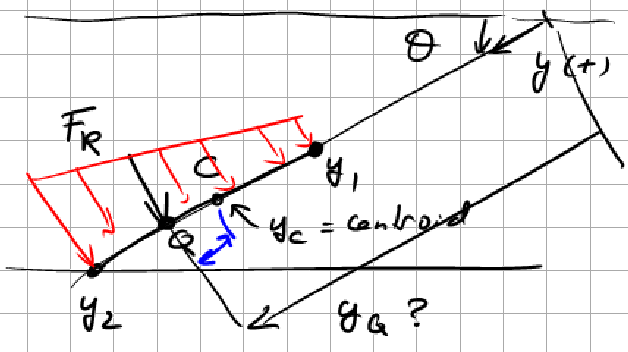
\includegraphics[width=0.33\textwidth]{Angled_Flat_Submerged_Surface_Pressure}
            \centering
        \end{Figure}
        
        Resultant force: $F_R = p_0 A + \rho g \sin{\theta} \,y_C A$
        
        Force is located at $y_Q = y_C + \frac{I_{xx,C}}{\frac{p_0 A}{\rho g \sin{\theta}} + y_C A}$
        
        For a rectangle with size $a$ in $x$-dir and $b$ in $y$-dir, $y_C = b/2$ and $I_{xx,C} = a b^3 / 12$.
        
        \fsheetlabel{Submerged curved body:}
        
        \begin{itemize}
            \item \textbf{Rule 1:} Horizontal force component is force on plane area formed by projecting curved surface onto vertical plane (\textit{e.g. use flat angled body above with $ \theta = \ang{0} $}).
            \item \textbf{Rule 2:} Vertical force component is weight of entire column of fluid above curved area (location can be found by doing FBD with weight of each piece @ respective centroids).
        \end{itemize}
    
        \fsheetlabel{Buoyancy:} Weight of the fluid displaced by an object directed upwards through centre of \textit{submerged} mass (e.g. $ F_B = \rho_f V g $). \textbf{Note:} If $ \rho_{f1} \gg \rho_{f2} $ (e.g. if $\rho_{f1}$ is for air, $\rho_{f2}$ is for water) then $ F_B = \left(\rho_{f1}V_1 + \rho_{f2}V_2\right)g \approx \rho_{f2}V_2g$.
        
        \fsheetlabel{Drag force @ terminal (settling) velocity:} $ F_D = \left( \rho_s - \rho_f \right) V g $ (you can solve for $ \rho_s $ if you have an expression for $ F_D $ already).
    \end{minipage}
    \vspace{2ex plus .5ex minus .5ex}
    %--------------------------------------
    
    %--------------------------------------
    \begin{minipage}{\columnwidth}\raggedright
        \subsection{Surface tension}
        
        \fsheetlabel{Energy to create interface:} $\delta W = \gamma \,dA$ where $\gamma$ is surface tension $\left[ \si{\joule\per\square\metre} \text{ or } \si{\newton\per\metre} \right]$.
        
        \fsheetlabel{Droplets on surfaces:} \textbf{hydrophilic} if $\theta < 90\degree$, \textbf{hydrophobic} if $\theta > 90\degree$.
        
        \fsheetlabel{Spreading coefficient:} $S = \gamma_{SG} - \left(\gamma_{SL} + \gamma_{LG}\right)$. $S>0$ $\Rightarrow$ film forms $\Rightarrow$ complete wetting. $S<0$ $\Rightarrow$ partial wetting $\Rightarrow$ drops.
        
        \fsheetlabel{Young-Laplace equation (droplet/bubble):} $p_{in} - p_{out} = 2\frac{\gamma}{R}$ where $R$ is radius of curvature.
        
        \fsheetlabel{Young-Laplace equation (capillary):} $p_{g} - p_{l} = \frac{2\gamma\cos{\left(\theta\right)}}{r}$, where $r$ is radius of capillary.
        
        $p_g - p_l > 0$ $\Rightarrow$ $\theta < \ang{90}$ $\Rightarrow$ CDN meniscus above water level.
        $p_g - p_l < 0$ $\Rightarrow$ $\theta > \ang{90}$ $\Rightarrow$ CUP meniscus below water level.
    \end{minipage}
    \vspace{2ex plus .5ex minus .5ex}
    %--------------------------------------
    
    %--------------------------------------
    \begin{minipage}{\columnwidth}\raggedright
        \subsection{That droplet question you missed earlier}
        
        Gosh dang-it man...
        
        \textbf{\textit{REMEMBER:}}
        
        \begin{Figure}
            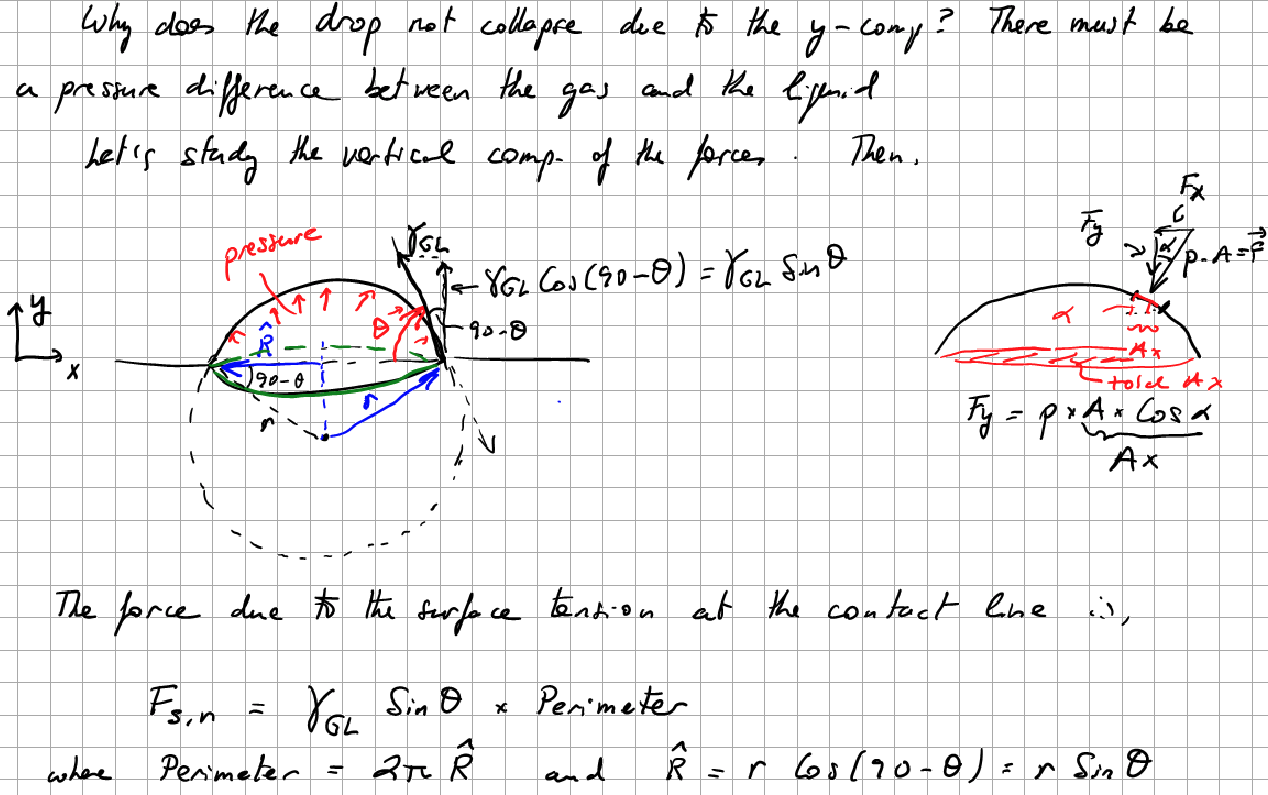
\includegraphics[width=\textwidth]{droplet_question}
            \centering
        \end{Figure}
    
        Gonna put this here again so you don't screw up again...
        
        \fsheetlabel{Energy to create interface:} $\delta W = \gamma \,dA$ where $\gamma$ is surface tension $\left[ \si{\joule\per\square\metre} \text{ or } \si{\newton\per\metre} \right]$.
        
        \fsheetlabel{Droplets on surfaces:} \textbf{hydrophilic} if $\theta < 90\degree$, \textbf{hydrophobic} if $\theta > 90\degree$.
        
        \fsheetlabel{Spreading coefficient:} $S = \gamma_{SG} - \left(\gamma_{SL} + \gamma_{LG}\right)$. $S>0$ $\Rightarrow$ film forms $\Rightarrow$ complete wetting. $S<0$ $\Rightarrow$ partial wetting $\Rightarrow$ drops.
        
        \fsheetlabel{Young-Laplace equation (droplet/bubble):} $p_{in} - p_{out} = 2\frac{\gamma}{R}$ where $R$ is radius of curvature.
    \end{minipage}
    \vspace{2ex plus .5ex minus .5ex}
    %--------------------------------------
    
    %--------------------------------------
    \begin{minipage}{\columnwidth}\raggedright
        \subsection{Fluid Dynamics}
        
        \fsheetlabel{Mass conservation:} For a fixed CV, $ \frac{d{m}_{CV}}{dt} = \dot{m}_{in} - \dot{m}_{out} $ where $ \dot{m} = \rho \dot{V} = \rho v_{avg} A $
        
        \fsheetlabel{Linear momentum conservation:} For a fixed CV, $ \Sigma F_x = \frac{dB_x}{dt} = \frac{dB_{x,CV}}{dt} + \dot{m}_{out} v_{x,out} - \dot{m}_{in} v_{x,in} $, where $ \Sigma F_x $ includes \textit{all} external body and surface forces, i.e. weight, pressure (gauge in most cases), viscous and reaction forces.
        
        \fsheetlabel{Specific enthalpy:} $ h = u + \frac{p}{\rho} $
        
        For solid, liquids, and ideal gases with constant $c_p$, $ h_2 - h_1 = c_p \left( T_2 - T_1 \right) $.
        
        \fsheetlabel{Energy conservation:} For a fixed CV, $ \frac{dE_{CV}}{dt} = \dot{Q}_{CV} - \dot{W}_{CV} + \dot{m}_i \left( h_i + \frac{v_i^2}{2} + g z_i \right) - \dot{m}_o \left( h_o + \frac{v_o^2}{2} + g z_o \right)$
        
        \fsheetlabel{Easy Bernoulli:} For \textbf{adiabatic}, \textbf{isothermal}, \textbf{incompressible}, \textbf{inviscid} fluids, and a fixed CV with one inlet and one outlet, $ \frac{p_i}{\rho} + \frac{v_i^2}{2} + g z_i = \frac{p_e}{\rho} + \frac{v_e^2}{2} + g z_e = \mathrm{constant} = H$ (\textbf{total head}).
        
        \fsheetlabel{Stagnation point:} Where the fluid's velocity is 0. If you see one, you should probably use Bernoulli somewhere.
    \end{minipage}
    \vspace{2ex plus .5ex minus .5ex}
    %--------------------------------------
    
    %--------------------------------------
    \begin{minipage}{\columnwidth}\raggedright
        \subsection{When we actually care about viscosity}
        
        Everything below is for circular pipes.
        
        \fsheetlabel{Reynolds Number:} Determines stability of flow. Defined as $ Re = \frac{\rho v L}{\mu} = \frac{\rho v_{avg} D}{\mu} = \frac{\mathrm{inertial \,forces}}{\mathrm{viscous \,forces}} $, where $ \rho $ is fluid's density, $ V = v_{avg} $ is characteristic (or average) velocity, $ L = D $ is characteristic length (or diameter), and $ \mu $ is kinematic viscosity.
        
        \fsheetlabel{Laminar Flow:}
        
        \begin{itemize}
            \item All particles move parallel.
            \item $ Re \leq 2100 $
            \item \fsheetlabel{Friction factor:} $f = \frac{64}{Re}$
            \item Velocity distribution inside pipe: $ v(r) = \frac{R^2}{4\mu} \left( \frac{\Delta p}{L} - \rho g \sin{\theta} \right) \left( 1 - \left( \frac{r}{R} \right)^2 \right)$.
            \item Velocity distribution inside \textit{horizontal} pipe: $ v(r=0) = v_{max} = \frac{R^2}{4\mu} \frac{\Delta p}{L} = 2v_{avg} $.
        \end{itemize}
    
        \fsheetlabel{Turbulent flow:}
        
        \begin{itemize}
            \item Freaking weird particle movement.
            \item Colebrook eq. (\textbf{unsolvable!}): $ \frac{1}{\sqrt{f}} = -2.0 \log{\left( \frac{\nicefrac{\varepsilon}{D}}{3.7} + \frac{2.51}{Re \sqrt{f}} \right)} $
            \item Within 2\% of Colebrook: $ \frac{1}{\sqrt{f}} \approx -1.8 \left( \left( \frac{\nicefrac{\varepsilon}{D}}{3.7} \right)^{1.11} + \frac{6.9}{Re} \right) $
        \end{itemize}
    
        \fsheetlabel{Steps for using the Moody Chart:}
        
        \begin{enumerate}
            \item Compute $Re$
            \item Compute $ \nicefrac{\varepsilon}{D} $ (both in metres!)
            \item Pick line on chart
        \end{enumerate}
    
        \fsheetlabel{Darcy-Weisbach formula:} $ \Delta p = f \cdot \frac{L}{D} \cdot \frac{1}{2} \rho v_{avg}^2 $
        
        \fsheetlabel{Hydrodynamic diameter:} $ D_h = \frac{4A_c}{P_{wetted}} $. Then, $ Re_{D_h} = \frac{\rho v_{avg} D_h}{\mu} $ and $ \Delta P = f \cdot \frac{L}{D_h} \cdot \frac{1}{2} \rho v_{avg}^2 $
    \end{minipage}
    \vspace{2ex plus .5ex minus .5ex}
    %--------------------------------------
    
    %--------------------------------------
    \begin{minipage}{\columnwidth}\raggedright
        \subsection{Bernoulli with viscosity effects}
        
        For an incompressible viscous fluid, and a CV with one inlet and one outlet,
        
        $$ \frac{p_1}{\rho g} + \frac{v_1^2}{2g} + z_1 + h_p = \frac{p_2}{\rho g} + \frac{v_2^2}{2g} + z_2 + h_T + \sum h_L $$
        
        where $ h = \frac{\Delta p}{\rho g} $ is some sort of head. Specifically:
        
        \fsheetlabel{Pump head:} $ h_P = \frac{\Delta p}{\rho g} = \frac{\dot{W}_P}{\dot{m}g} $
        
        \fsheetlabel{Turbine head:} $ h_T = \frac{\Delta p}{\rho g} = \frac{\dot{W}_T}{\dot{m}g} $
        
        \fsheetlabel{Head losses:} $ \sum h_L = \sum f \frac{L}{D} \frac{v^2}{2g} $
    \end{minipage}
    \vspace{2ex plus .5ex minus .5ex}
    %--------------------------------------
    
    %--------------------------------------
    \begin{minipage}{\columnwidth}\raggedright
        \subsection{Important unit conversions}
        
        \fsheetlabel{Energy, work:}
        
        $\SI{1}{\britishthermal} = \SI{778.169}{\feet\poundsforce}$
        
        \fsheetlabel{Temperature:}
        
        $T(\si{\degreeFahrenheit}) = \frac{9}{5} T(\si{\degreeCelsius}) + 32$
        
        $T(\si{\degreeCelsius}) = \frac{5}{9}(T(\si{\degreeFahrenheit}) - 32)$
        
        $T(\si{\kelvin}) = T(\si{\degreeCelsius}) + 273.15$
        
        $T(\si{\rankine}) = T(\si{\degreeFahrenheit}) + 459.67$
        
        $T(\si{\rankine}) = \frac{9}{5} T(\si{\kelvin})$
        
        \fsheetlabel{Volume:}
        
        $\SI{1}{\cubic\metre} = \SI{1000}{\liter}$
        
        $\SI{1}{\cubic\centi\metre} = \SI{1}{\milli\liter}$
        
        \fsheetlabel{Mass, force:}
        
        $\SI{1}{\poundsmass} = \frac{1}{\num{32.174}}\si{\slug} = \frac{\SI{1}{\poundsforce}}{\SI{32.174}{\feet\per\second\squared}}$
    \end{minipage}
    \vspace{2ex plus .5ex minus .5ex}
    %--------------------------------------
    
    %--------------------------------------
    \begin{minipage}{\columnwidth}\raggedright
        \subsection{Important constants}
        
        \fsheetlabel{Universal Gas Constant:}
        
        \vspace{-0.5cm}
        \begin{align*}
            \bar{R} &= \SI{8.31434}{\joule\per\mole\per\kelvin} \\
                    &= \SI{1.9858}{\britishthermal\per\poundsmole\per\rankine} \\
                    &= \SI{1545.35}{\feet\poundsforce\per\poundsmole\per\rankine} \\
                    &= \SI{10.73}{\AbsPressurePerSquareInch\feet\cubed\per\poundsmole\per\rankine}
        \end{align*}
        \vspace{-0.5cm}
        
        \fsheetlabel{Water density at $\SI{4}{\celsius}$:} $\rho_{H_2 O, \SI{4}{\celsius}} = \SI{1000}{\kilogram\per\cubic\metre}$
    \end{minipage}
    \vspace{2ex plus .5ex minus .5ex}
    %--------------------------------------
    
    %--------------------------------------
    \begin{minipage}{\columnwidth}\raggedright
        \subsection{Important equations I constantly forget}
        
        \fsheetlabel{Spheres:} $ V = \frac{4}{3} \pi r^3 $, $ A = 4\pi r^2 $.
        
        \fsheetlabel{Cylinders:} $ V = \pi r^2 h $, $ A = 2\pi r h + 2\pi r^2 $.
    \end{minipage}
    \vspace{2ex plus .5ex minus .5ex}
    %--------------------------------------
    
    % You can even have references
    % \rule{0.3\linewidth}{0.25pt}
    % \scriptsize
    % \bibliographystyle{abstract}
    % \bibliography{refFile}
    \end{multicols*}
\end{document}